\section{Preliminaries}
\begin{figure*}[t!]
    \centering
    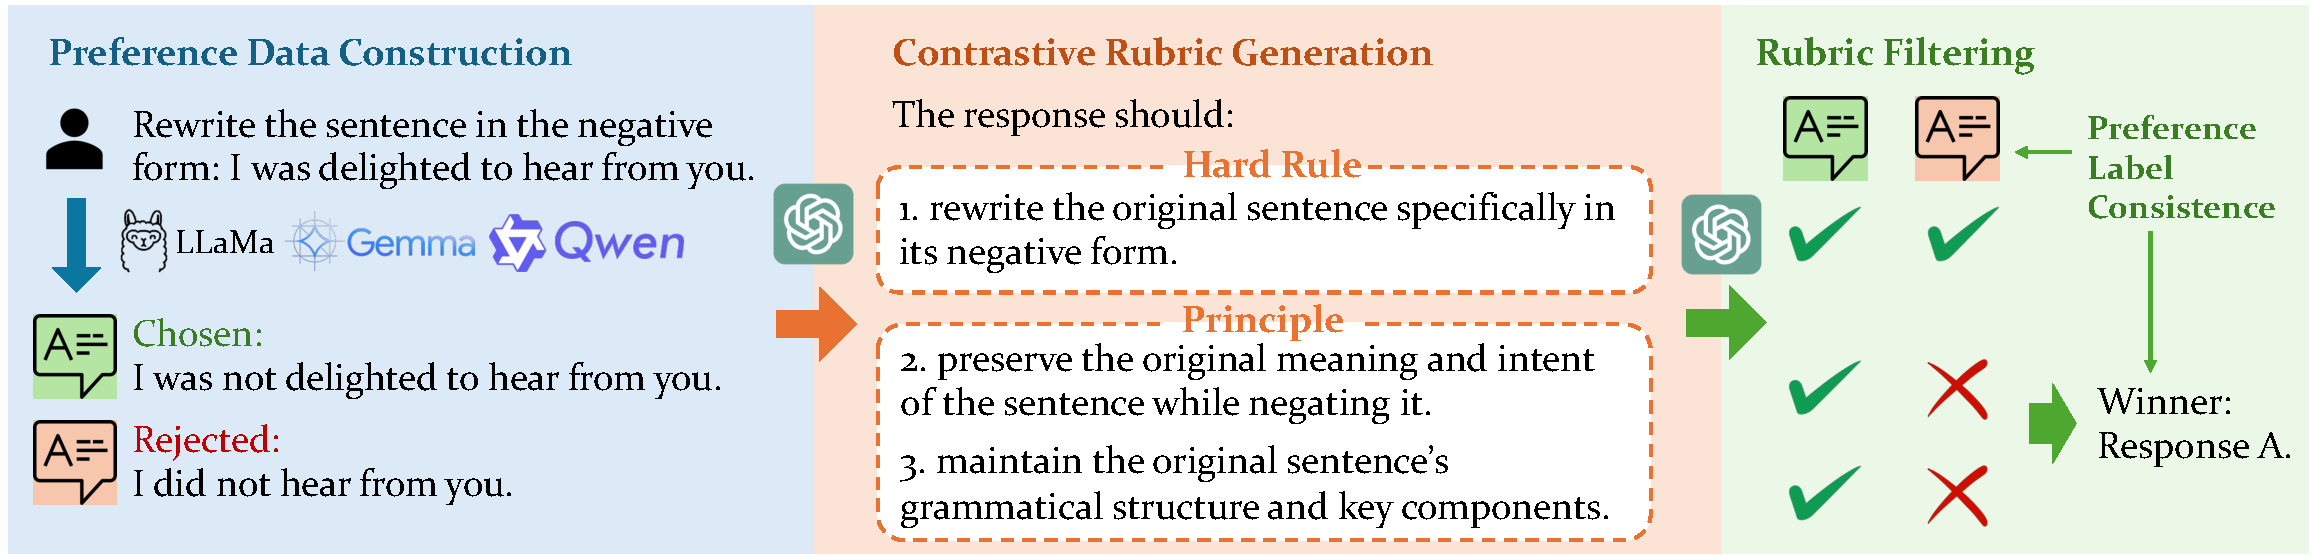
\includegraphics[width=0.95\textwidth]{figures/framework.pdf}
    \caption{\centering Overall Framework for Synthetic Rubric Generation in \dataset{}. \vspace{-1ex}}
    \label{fig:framework}
\end{figure*}

\noindent \textbf{Rubrics.}
We define rubrics as a structured set of evaluation criteria tailored to a given prompt. 
Formally, let $x$ denote an input prompt and $\hat{y}$ a model-generated response. 
A rubric $\mathcal{R}(x)$ is represented as a collection of $k$ criteria 
$\mathcal{R}(x) = \{c_i\}_{i=1}^k$,
where each $c_i$ denotes a rubric description specifying an aspect of response quality (e.g., factual correctness, reasoning soundness, style).  


\noindent \textbf{Rubrics-based Reward Models.}
Building on prior work in pairwise reward modeling~\citep{liu2025pairjudge,chen2025rm,guo2025reward,xu2025unified},  
we focus on a comparative setting where the goal is to evaluate the relative quality of two candidate responses.  
Given a prompt $x$ and two samples $(\hat{y}_1, \hat{y}_2)$,  
a pairwise rubric-based reward function is defined as
\begin{equation}
\setlength{\abovedisplayskip}{5pt}
\setlength{\belowdisplayskip}{5pt}
\nonumber
   \text{reward}_{\text{pair}}(x,\hat{y}_1,\hat{y}_2) 
   = r_{\theta}\big(x,\hat{y}_1,\hat{y}_2;\{c_i\}_{i=1}^k \big),
\end{equation}
where $\text{reward}$ is the binary preference label, $r_\theta$ is the reward model that integrates rubric criteria $\{c_i\}$ when producing a preference judgment.  

The overall framework for \dataset{} is in Figure \ref{fig:framework}. Our overall objective is two-fold:  
(1) constructing a rubric dataset $\mathcal{D}_{\text{rubric}}$ to train a generation model $g_{\theta}$ that automatically synthesizes rubrics $\mathcal{R}(x)$ given a prompt $x$; and  
(2) building a reward modeling dataset $\mathcal{D}_{\text{rm}}$ to train a rubric-guided reward model $r_{\phi}$ capable of producing reliable and interpretable pairwise judgments.  
This two-stage formulation decomposes evaluation into \emph{rubric generation} and \emph{rubric-conditioned reward prediction}, bridging human-aligned criteria and automated preference modeling.
% Our goal is two-fold:  
% (i)  constructing the dataset $\mathcal{D}_{\text{rubric}}$ for training the rubric generation model $f_{\theta}$, enabling the automatic synthesis of rubrics $\mathcal{R}(x)$ given prompts $x$.  
% (ii) constructing the dataset $\mathcal{D}_{\text{rm}}$ for training the rubric-based reward model $g_{\phi}$ so that it can produce reliable, rubric-grounded pairwise judgments.  



\section{\dataset{}}
\label{sec:dataset}
\subsection{Data Construction}
\label{sec:data_construct}
\textbf{Data Sources.} To generate high-quality rubrics that generalize across tasks and domains, we integrate a range of publicly available preference and instruction-tuning datasets, 
balancing general-domain data with domain-specific resources.  
Specifically, our dataset draws from the following sources:
\begin{itemize}[leftmargin=0.4cm,itemsep=0.1pt]
    \item \textbf{UltraFeedback}~\citep{cui2024ultrafeedback}, which aggregates preference annotations from 
    \emph{Evol-Instruct}~\citep{xu2024wizardlm}, \emph{UltraChat}~\citep{ultrachat}, \emph{ShareGPT}~\citep{sharegpt}, and \emph{TruthfulQA}~\citep{lin-etal-2022-truthfulqa}.
    \item \textbf{Magpie}~\citep{xu2025magpie}: a large-scale synthetic alignment dataset generated by self-prompting LLMs across diverse domains.
    % \item \textbf{HelpSteer3}~\citep{wang2025helpsteer3}, a large-scale human-annotated dataset designed for alignment with helpfulness preferences.
    \item \textbf{Skywork-Preference}~\citep{liu2024skywork}, which integrates data from \emph{HelpSteer2}~\citep{wang2024helpsteer} and \emph{OffsetBias}~\citep{offsetbias}.
    \item \textbf{Synthetic-IF}~\citep{lambert2025tulu}, a collection of human preference judgments tailored for verifiable instruction-following.
    \item \textbf{MegaScience}~\citep{fan2025megascience}, a specialized corpus spanning multiple scientific domains including physics, biology, and chemistry.
    \item \textbf{Medical-o1}~\citep{chen2024huatuogpt}, a medical SFT dataset curated for diagnostic reasoning tasks.
\end{itemize}


% \begin{figure}[t!]
%     \centering
%     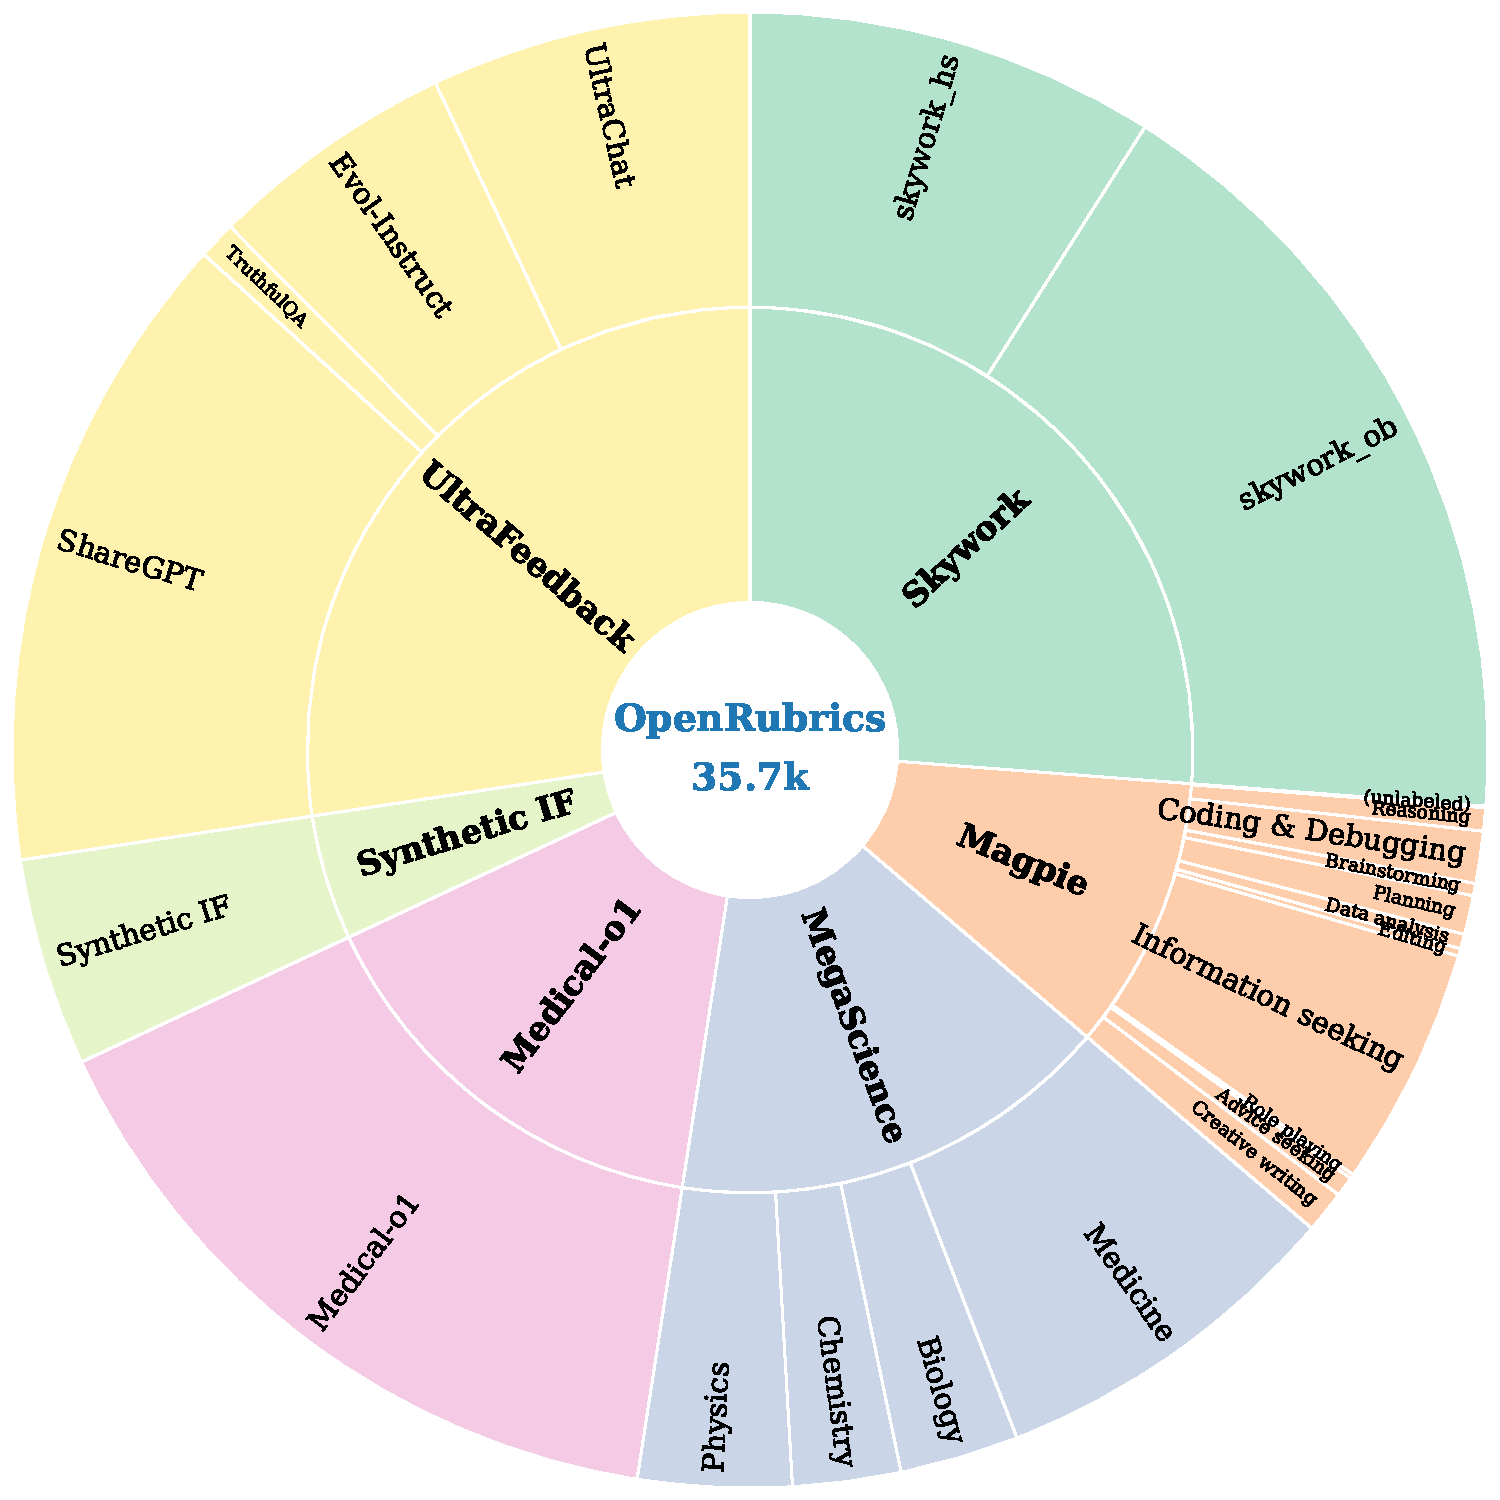
\includegraphics[width=0.5\columnwidth]{figures/pie_chart.pdf}
%     \caption{\color{red} Data statistics.}
%     \label{fig:pie_chart}
% \end{figure}
\begin{figure*}[t!]
    \centering
    \begin{subfigure}{0.47\linewidth}
        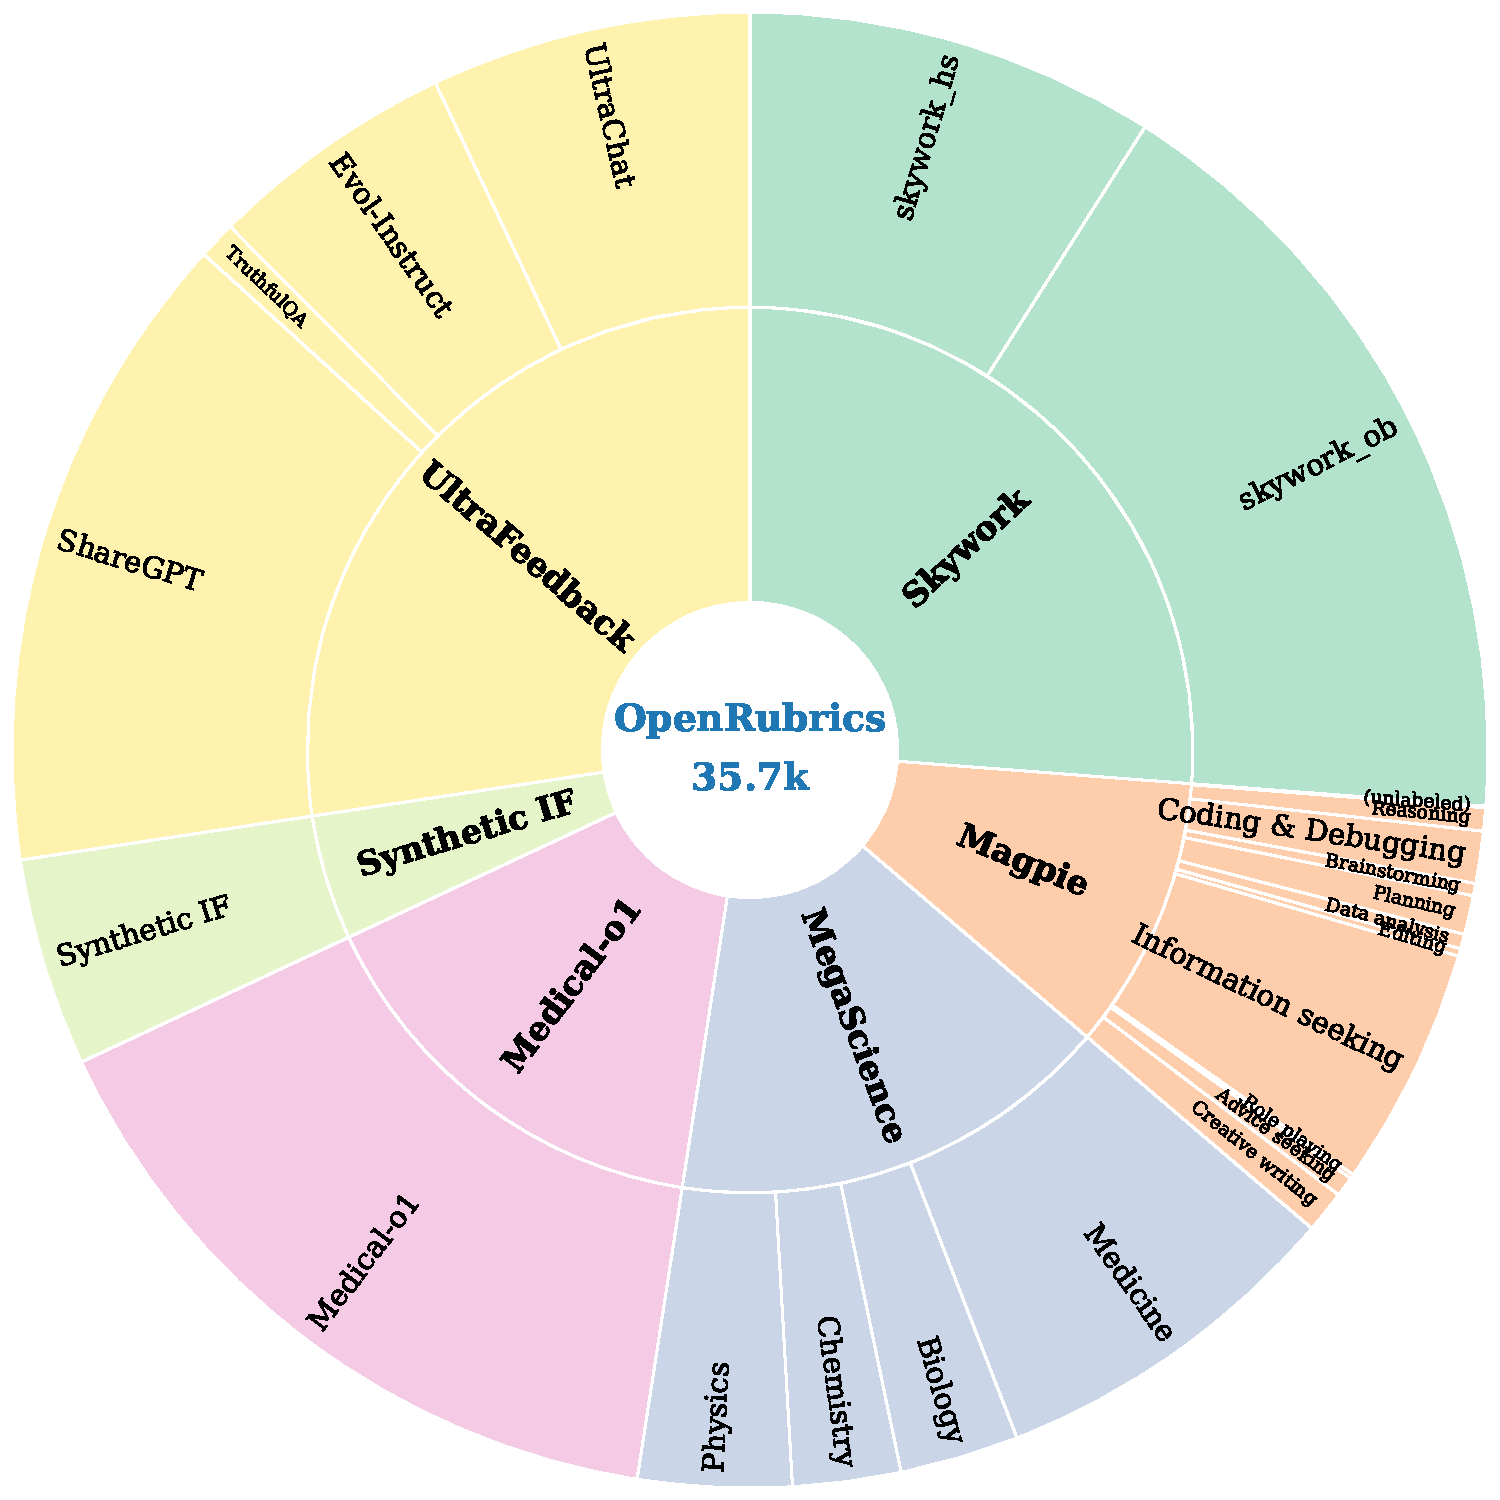
\includegraphics[width=\linewidth]{figures/pie_chart.pdf}
        \caption{\centering The data distribution for \dataset{} (in \# instructions).}
        \label{fig:pie_chart}
    \end{subfigure}
    \hfill
    \begin{subfigure}{0.51\linewidth}
        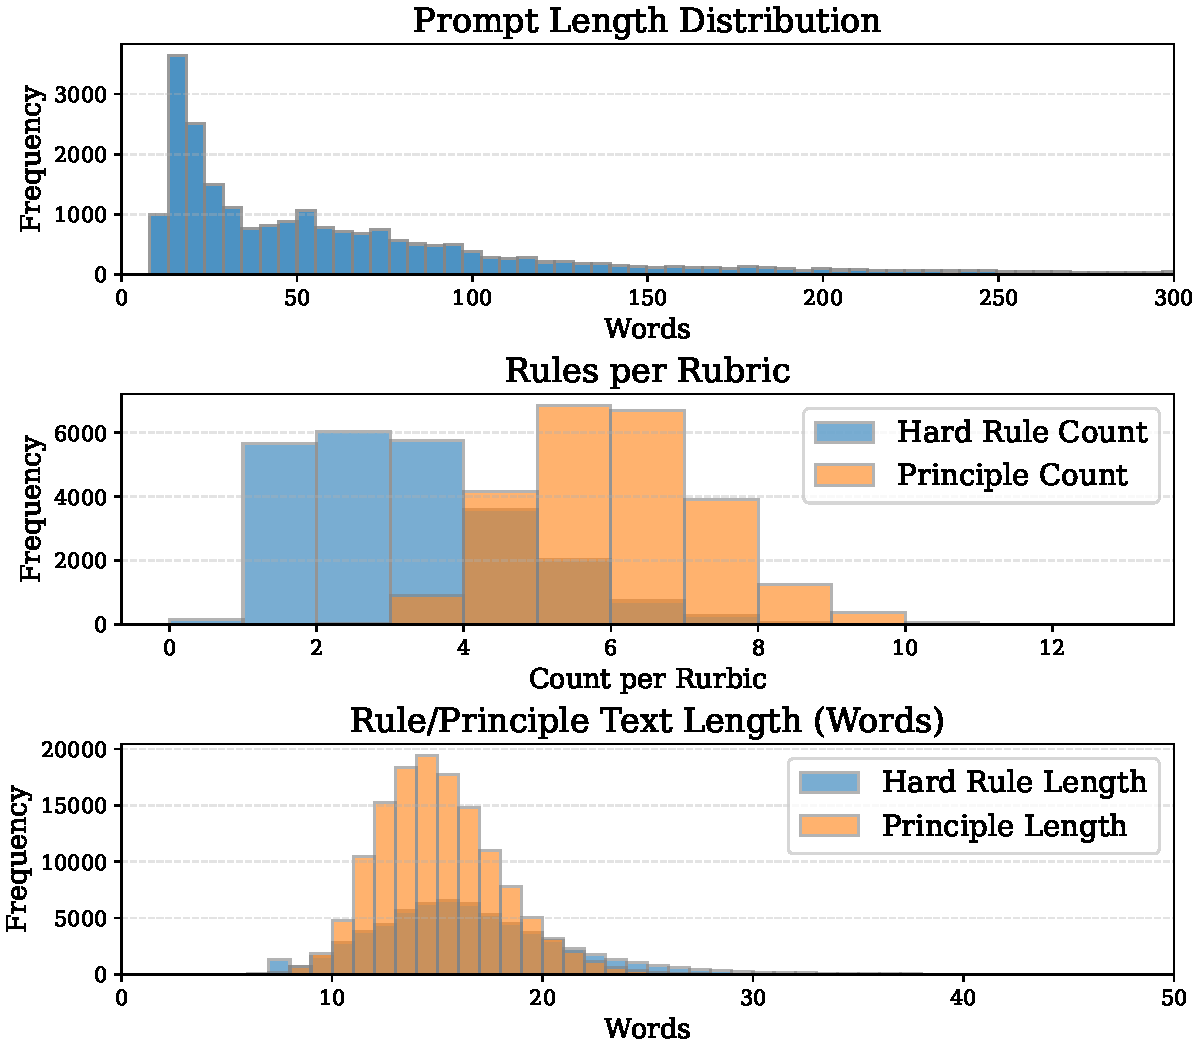
\includegraphics[width=\linewidth]{figures/hist.pdf}
        \caption{\centering The distribution for the length of prompts and rubrics, as well as the number of rubrics.}
        \label{fig:hist}
    \end{subfigure}
    % \vspace{-1.5ex}
    \caption{\centering Statistics Overview of \dataset{}.\vspace{-2ex}}
    \label{fig:stats}
\end{figure*}

\noindent \textbf{Preference Data Construction.}  
To build preference data for rubric generation and judge training (see Sec.~\ref{sec:rm_train}), we reuse existing preference and SFT datasets with tailored processing.
For \textbf{UltraFeedback}, we select the highest-scoring response as the \emph{chosen} and the lowest as the \emph{rejected}.
For \textbf{MegaScience}, and \textbf{Medical-o1}, we generate multiple responses using \textit{Qwen-3-8B/14B}~\citep{yang2025qwen3}, \textit{Llama-3.1-8B}~\citep{grattafiori2024llama}, and \textit{Gemma-3-12B}~\citep{team2025gemma}, selecting one from each model.
For \textbf{Synthetic-IF}, responses satisfying all verification functions are labeled as \emph{chosen}, and others as \emph{rejected}.
For the \textbf{MegaScience} and \textbf{Medical-o1} datasets, we employ an ensemble of open-source reward models: \textit{Athene-RM-8B}~\citep{Athene2024} and \textit{Skywork-Reward-V2-Llama-3.1-8B-40M}~\citep{liu2025skywork} to rank responses and form best–worst preference pairs.


% \subsection{Data Sources}
% List data source:
% - ultrafeedback~\citep{cui2024ultrafeedback}
%     - evol instruct
%     - ultrachat
%     - shareGPT
%     - truthfulQA
    
% - tulu 2.5~\citep{ivison2024unpacking}
%     - alpaca\_farm
%     - chatbot\_arena
%     - argilla
%     - capybara
%     - stackexchange
%     - nectar
%     - orca
% - helpsteer3~\citep{wang2025helpsteer3}
% - skywork~\citep{liu2024skywork}
%     - helpsteer2
%     - offsetbias
% - IF~\citep{lambert2025tulu}

% Skywork-reward~\citep{liu2025skywork}, Athene \citep{Athene2024}

% \~20k

\subsection{Rubrics Synthesis}
\label{sec:rubrics_gen}
After collecting a diverse set of preference pairs, our objective is to construct a set of rubrics that serve as \emph{anchors} to guide   reward modeling.
To comprehensively represent different types of constraints while preserving discriminative granularity, we categorize rubrics into two  types:
(1) \textbf{Hard Rules}, which capture explicit requirements stated in the user’s prompt; and
(2) \textbf{Principles}, which describe higher-level qualitative aspects such as reasoning soundness, factuality, or stylistic coherence.
We then introduce two strategies for generating high-quality rubrics as follows:  

% \noindent \textbf{Contrastive Rubric Generation.} 
% Given a preference dataset
% $
% \mathcal{D}=\left\{\left(x_i, \hat{y}_i^{+}, \hat{y}_i^{-}\right)\right\}_{i=1}^N,
% $
% where $x_i$ is the prompt and $\hat{y}_i^{+}$ and $\hat{y}_i^{-}$ denote the preferred and displeased responses, respectively. Our objective is to infer rubrics $\mathcal{R}\left(x_i\right)$ that capture qualities a good response should satisfy and the criteria by which one response is preferred over another, using $\hat{y}_i^{+}$ and $\hat{y}_i^{-}$ as guidance.
% % explain why one response is preferred over the other.
% Formally, we prompt an instruction-tuned LLM $h_\psi$ as 
% $
% \mathcal{R}\left(x_i\right) \sim h_\psi\left(x_i, \hat{y}_i^{+}, \hat{y}_i^{-}, \ell_i\right),
% $
% where $\ell_i$ is the preference label.
% The generator is asked to produce a set of discriminative evaluation criteria $\mathcal{R}\left(x_i\right)=\left\{c_{i, 1}, \ldots, c_{i, k_i}\right\}$,
% where each $c_{i, j}$ describes a specific aspect.
% This setting encourages the model to discover rubric dimensions that are both task-sensitive and preference-aligned.

\noindent \textbf{Contrastive Rubric Generation.} 
Given a preference dataset
$
\mathcal{D}=\left\{\left(x_i, \{\hat{y}_{i,m}\}_{m=1}^{M_i}, \{\ell_{i,m}\}_{m=1}^{M_i}\right)\right\}_{i=1}^N,
$
where $x_i$ is the prompt, $\{\hat{y}_{i,m}\}_{m=1}^{M_i}$ and $\{\ell_{i,m}\}_{m=1}^{M_i}$ denotes a list of candidate responses and their corresponding preference signals, respectively.
The preference signal $\ell_{i,m}$ can be a real-valued score when available, or a binary chosen--rejected label.
We unify both cases by constructing a strictly ordered list in descending preference:
$
\hat{y}_{i,1}\succ \hat{y}_{i,2}\succ \cdots \succ \hat{y}_{i,M_i},
$
where the order is induced by $\ell$.
In particular, when only chosen--rejected labels are available, we simply set $M_i=2$ with $\hat{y}_{i,1}$ as chosen and $\hat{y}_{i,2}$ as rejected.
Our objective is to infer rubrics $\mathcal{R}(x_i)$ that capture qualities a good response should satisfy and the criteria that explain preference differences across the list, leveraging rich and fine-grain supervision from the comparisons.
Formally, we prompt an instruction-tuned LLM $h_\psi$ as
$
\mathcal{R}(x_i) \sim h_\psi\!\left(x_i, \{\hat{y}_{i,m}\}_{m=1}^{M_i}, \{\ell_{i,m}\}_{m=1}^{M_i}\right).
$
The generator is asked to produce a set of discriminative evaluation criteria
$\mathcal{R}(x_i)=\left\{c_{i,1}, \ldots, c_{i,k_i}\right\}$,
where each $c_{i,j}$ describes a specific aspect and is expected to distinguish higher-preference responses from lower-preference ones.
This listwise setting encourages the model to discover rubric dimensions that are both task-sensitive and preference-aligned, while exploiting any available fine-grained preference information.


% \noindent \textbf{Rubric Filtering with Preference-label Consistency.}
% Not all generated rubrics faithfully capture the human preference signal.
% To ensure reliability, we conduct a consistency-based filtering step via prompting the LLM $h_\psi$ again.
% For each triplet ($x_i, \hat{y}_i^{+}, \hat{y}_i^{-}$), we concatenate the full rubric $\mathcal{R}\left(x_i\right)$ into the context and ask the model to predict which response better aligns with the rubric
% $
% \hat{l}_i=h_\psi\left(x_i, \mathcal{R}\left(x_i\right), \hat{y}_i^{+}, \hat{y}_i^{-}\right),
% $
% % where $\hat{l}_i = (\hat{r}_i, \hat{\ell}_i)$ is the final prediction, $\hat{r}_i$ denotes the prediction rationale and $\hat{\ell}_i$ denotes the predicted preference.
% where $\hat{l}_i = (\hat{r}_i, \hat{\ell}_i)$ denotes the prediction rationale and the predicted preference, respectively.
% For pairwise judging, we retain only those rubrics that lead to predictions consistent with the original human label $\ell_i$:
% \begin{equation}
% \setlength{\abovedisplayskip}{5pt}
% \setlength{\belowdisplayskip}{5pt}
% \mathcal{R}^*\left(x_i\right)= \begin{cases}\mathcal{R}\left(x_i\right), & \text { if } \hat{\ell}_i=\ell_i, \\ \emptyset, & \text { otherwise. }\end{cases}
% \end{equation}

% For listwise judging settings, where a single prompt is associated with multiple candidate responses, we decompose the task into multiple pairwise comparisons.
% In this case, we retain a rubric if it yields preference predictions consistent with human labels in at least $50\%$ of the induced pairwise comparisons, allowing robustness to occasional ambiguity while preserving discriminative power.

% This yields a collection of high-quality rubrics that are both interpretable and empirically consistent with human preferences.
% The final \emph{rubrics-conditioned preference dataset} combines prompts, paired responses, and their verified rubrics as 
% $
% \mathcal{D}_{\text {rubric }}=\left\{\left(x_i, \hat{y}_i^{+}, \hat{y}_i^{-}, \mathcal{R}^*(x_i)\right)\right\}_{i=1}^M.
% $


\noindent \textbf{Rubric Filtering with Preference-label Consistency.}
Not all generated rubrics faithfully capture the human preference signal.
To ensure reliability, we perform a consistency-based filtering step by prompting the same instruction-tuned LLM $h_\psi$ again.
Specifically, for each prompt $x_i$ with an ordered response list $\{\hat{y}_{i,m}\}_{m=1}^{M_i}$, we construct a set of induced pairwise comparisons
$
\mathcal{P}_i=\{(a,b)\mid 1\le a<b\le M_i\},
$
where the human preference label for each pair is $\ell_{i,(a,b)}=1$ (i.e., $\hat{y}_{i,a}\succ \hat{y}_{i,b}$).
When the original data only provides chosen--rejected labels, we have $M_i=2$ and thus $|\mathcal{P}_i|=1$.
Next, we concatenate the full rubric $\mathcal{R}(x_i)$ into the context and ask the model to judge each induced pair:
\begin{equation}
\hat{l}_{i,(a,b)} = h_\psi\!\left(x_i, \mathcal{R}(x_i), \hat{y}_{i,a}, \hat{y}_{i,b}\right),
\end{equation}
where $\hat{l}_{i,(a,b)}=(\hat{r}_{i,(a,b)}, \hat{\ell}_{i,(a,b)})$ denotes the prediction rationale and the predicted preference, respectively.
A rubric is considered reliable for prompt $x_i$ only if it yields preference predictions consistent with human labels on the induced pair set:
\begin{equation}
\mathrm{Acc}_i
=
\frac{1}{|\mathcal{P}_i|}
\sum_{(a,b)\in\mathcal{P}_i}
\mathbb{I}\!\left[\hat{\ell}_{i,(a,b)}=\ell_{i,(a,b)}\right]
\ \ge\ \tau,
\end{equation}
where $\tau$ is a threshold (we use $\tau=0.5$).
% 
Finally, for each induced pair $(a,b)\in\mathcal{P}_i$, we retain the rubric-conditioned training instance only if
(i) the rubric passes the group-level verification ($\mathrm{Acc}_i\ge\tau$), and
(ii) the current pairwise prediction is correct ($\hat{\ell}_{i,(a,b)}=\ell_{i,(a,b)}$).
Formally,
\begin{equation}
\mathcal{R}^*_{i,(a,b)} =
\begin{cases}
\mathcal{R}(x_i), & \text{if} \quad \mathrm{Acc}_i \ge \tau \quad \text{and} \quad \hat{\ell}_{i,(a,b)}=\ell_{i,(a,b)},\\
\emptyset, & \text{otherwise.}
\end{cases}
\end{equation}
This yields a collection of high-quality rubrics that are both interpretable and empirically consistent with human preferences.
The final \emph{rubrics-conditioned preference dataset} is constructed as a pairwise one
\begin{align}
\mathcal{D}_{\text{rubric}}
&=
\left\{
\left(x_i, \hat{y}_{i,a}, \hat{y}_{i,b}, \ell_{i,(a,b)}, \mathcal{R}^*_{i,(a,b)}\right)
\ \middle|\ 
i\in[N],\ (a,b)\in\mathcal{P}_i,\ \mathcal{R}^*_{i,(a,b)}\neq\emptyset
\right\} \\
&\triangleq
\{(x_i,\hat{y}_i^+,\hat{y}_i^-,\mathcal{R}^*(x_i))\}_{i=1}^M.
\end{align}
Namely, we flatten and re-index all retained pairs to obtain the pairwise dataset,
where new instance corresponds to one retained $(i,(a,b))$ with $\hat{y}_i^+=\hat{y}_{i,a}$ and $\hat{y}_i^-=\hat{y}_{i,b}$.




\begin{figure}[t]
  \centering
   \vspace{-1ex}
  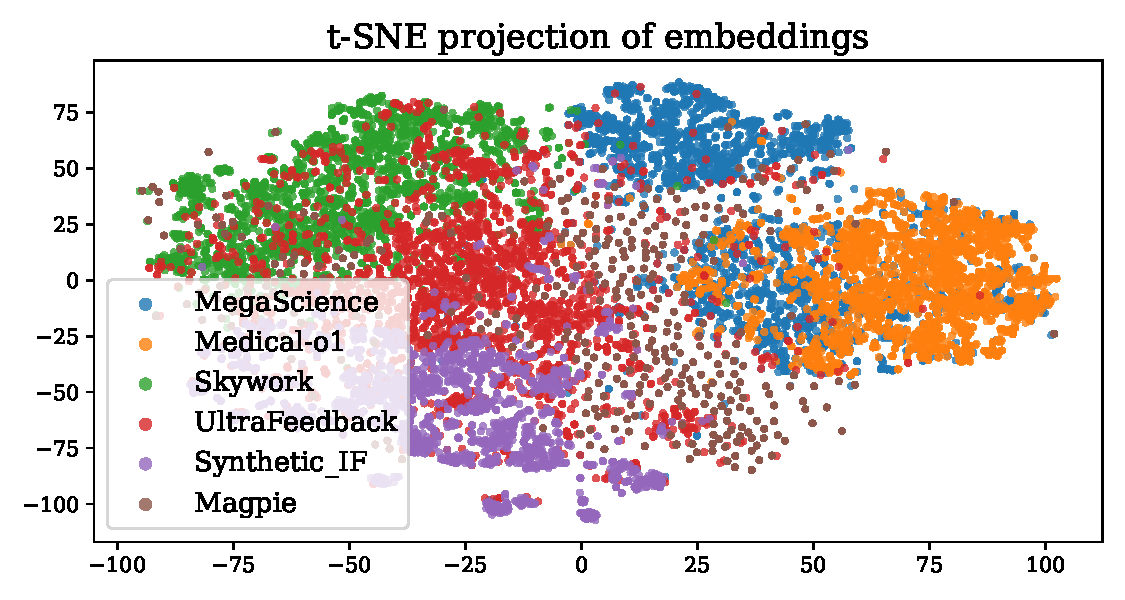
\includegraphics[width=0.7\linewidth]{figures/tsne_plot_v2.pdf}
  \caption{The T-SNE plot for embeddings of prompts. \vspace{-2ex}}
  \label{fig:tsne_plot}
\end{figure}

% \begin{wrapfigure}{r}{8.4cm}
% \vspace{-2ex}
% % \centering
% \includegraphics[width=0.9\linewidth]{figures/tsne_plot.pdf}
% \vspace{-3ex}
% \caption{The T-SNE plot for the embeddings of prompts.\vspace{-6ex}}
% \label{fig:tsne_plot}
% \end{wrapfigure}
\noindent \textbf{Rubric Statistics Overview.}
We analyze the curated rubric set along three axes: (1) domain coverage (instruction following, reasoning, general helpfulness; Figure~\ref{fig:pie_chart}); (2) the balance between \emph{hard rules} and \emph{principles} as well as the length of prompts and rubrics (Figure~\ref{fig:hist}); and (3) semantic diversity of prompt topics, visualized via t-SNE on embeddings from Qwen-3-Embedding-0.6B~\citep{zhang2025qwen3} (Figure~\ref{fig:tsne_plot}). 
These statistics confirm that the synthesized rubrics provide comprehensive, yet discriminative coverage, forming a foundation for rubric-based reward modeling.


\subsection{Reward Model Training and Inference}
\label{sec:rm_train}
After collecting the rubrics-based dataset, we proceed to develop a rubric generation model that outputs evaluation rubrics and a reward model \modelname{} that generates final preference labels.

\noindent \textbf{Rubric Generation.}
We first fine-tune $g_\theta$ to generate rubrics $\mathcal{R}^*$ conditioned on the prompt $x$. Given the dataset $\mathcal{D}_{\text{rubric}} = \{(x_i, \hat{y}_i^{+}, \hat{y}_i^{-}, \mathcal{R}^*(x_i))\}_{i=1}^{M}$, we optimize the standard cross-entropy objective:
% We first train a rubric generation model $g_\theta$ to produce structured evaluation rubrics conditioned on the prompt and paired responses.  
% Formally, given a dataset 
% $\mathcal{D}_{\text{rubric}}
% = \{(x_i, \hat{y}_i^{+}, \hat{y}_i^{-}, \mathcal{R}^*(x_i))\}_{i=1}^{M}$,
% where $\mathcal{R}^*(x_i)$ denotes the reference rubric associated with the prompt,  
% the model $g_\theta$ is trained via supervised fine-tuning (SFT) with the standard next-token cross-entropy loss:

\begin{small}
\begin{equation}
\setlength{\abovedisplayskip}{-5pt}
\setlength{\belowdisplayskip}{5pt}
\mathcal{L}_{\text{SFT}}^{\text{rubric}}
= -\,\mathbb{E}_{(x, \hat{y}^{+}, \hat{y}^{-}, \mathcal{R}^*) \in \mathcal{D}_{\text{rubric}}}
\sum_{t=1}^{|\mathcal{R}^*|}
\log p_\theta \big(\mathcal{R}^*_t \mid x, \mathcal{R}^*_{<t}\big).
\nonumber
\end{equation}
\end{small}


% This objective teaches the model to generate detailed, domain-relevant rubrics that encode evaluation criteria from the user-provided prompt, which can be subsequently used in reward modeling.
\noindent \textbf{Reward Model Training.}
We then train the reward model $r_\phi$ to predict preference labels $\hat{l}$ using the generated rubrics. Using $\mathcal{D}_{\text{rm}} = \{(x_i, \hat{y}_i^{+}, \hat{y}_i^{-}, \mathcal{R}^*(x_i), \hat{l}_i)\}_{i=1}^{M}$, we optimize $r_\phi$ to predict $\hat{l}$ conditioned on the prompt, response pair, and rubric:

\begin{small}
\begin{equation}
\setlength{\abovedisplayskip}{-8pt}
\setlength{\belowdisplayskip}{5pt}
\mathcal{L}_{\text{SFT}}^{\text{rm}}
= -\,\mathbb{E}_{\mathcal{D}_{\text{rm}}}
\sum_{t=1}^{|\hat{l}|}
\log p_\phi \big(\hat{l}_t \mid x, \hat{y}^{+}, \hat{y}^{-}, \mathcal{R}^*(x), \hat{l}_{<t}\big).
\nonumber
\end{equation}
\end{small}
% \paragraph{Reward Model Training.}
% Using the synthesized rubrics, we then train the reward model $r_\phi$ on
% $\mathcal{D}_{\text{rm}}
% = \{(x_i, \hat{y}_i^{+}, \hat{y}_i^{-}, \mathcal{R}^*(x_i), \hat{l}_i)\}_{i=1}^{M}$. 
% The model is also optimized via SFT to predict the label tokens $\hat{l}_i$ conditioned on the prompt, response pair, and rubric:

% \begin{small}
% \begin{equation}
% \mathcal{L}_{\text{SFT}}^{\text{rm}}
% = -\,\mathbb{E}_{\mathcal{D}_{\text{rm}}}
% \sum_{t=1}^{|\hat{l}|}
% \log p_\phi \big(\hat{l}_t \mid x, \hat{y}^{+}, \hat{y}^{-}, \mathcal{R}^*(x), \hat{l}_{<t}\big).
% \end{equation}
% \end{small}
    


\noindent \textbf{Inference.}
At inference time, given a pairwise test instance $(x, y^{\text{A}}, y^{\text{B}})$,  
\modelname{} performs a two-stage process to predict the final preference label:
(1) the rubric generator produces (or retrieve a cached) rubric conditioned on the instruction $x$ as $\hat{\mathcal{R}}(x) = g_\theta(x)$; (2) the reward model then predicts the verdict over candidate responses $(y^{\text{A}}, y^{\text{B}})$ conditioned on the generated rubric from two possible labels $\mathcal{C} = \{\text{A is better}, \text{B is better}\}$:

% \modelname{} performs a two-stage process to predict the final preference label: 
% (1) the rubric generator first produces $\hat{\mathcal{R}}(x) = g_\theta(x, y^{\text{A}}, y^{\text{B}})$;  
% (2) the reward model then predicts the verdict conditioned on the generated rubric from two possible labels $\mathcal{C} = \{\text{A is better}, \text{B is better}\}$:
% 
\begin{small}
\begin{equation}
\setlength{\abovedisplayskip}{4pt}
\setlength{\belowdisplayskip}{5pt}
\hat{l}
= \arg\max_{k \in \mathcal{C}}
p_\phi \big(k \mid x, y^{\text{A}}, y^{\text{B}}, \hat{\mathcal{R}}(x)\big).
\nonumber
\end{equation}
\end{small}
This ensures that the judgment from \modelname{} is explicitly grounded in rubric criteria.


% \subsection{Reward Model Training and Inference}
% \label{sec:rm_train}

% \paragraph{Training Rubric Generation Model.}
% $$
% \mathcal{D}_{\text {rubric }}=\left\{\left(x_i, \hat{y}_i^{+}, \hat{y}_i^{-}, \mathcal{R}^*(x_i)\right)\right\}_{i=1}^M.
% $$

% \paragraph{Training \modelname{}.}
% $$
% \mathcal{D}_{\text{rm}}=\left\{\left(x_i, \hat{y}_i^{+}, \hat{y}_i^{-}, \mathcal{R}^*(x_i), \hat{l}_i\right)\right\}_{i=1}^M.
% $$